\documentclass[11pt,a4paper]{article}
% =====================================================================
% PLOS NTD revision v3 (page-audit).
% PROVENANCE: This LaTeX manuscript source was reconstructed from the June 26, 2026
% manuscript PDF and user-supplied manuscript text. It is not the original authoring
% source. Revision v3 was derived from the preserved working state of revision v2 after
% a full page-by-page audit of the 17-page review PDF.
% Numbers are reused verbatim from the frozen committed reports (no recomputation).
% Unresolved administrative metadata are tracked in submission_blockers_v3.md, not in
% the manuscript body. Not for submission until the authors confirm those items.
% =====================================================================
\usepackage[utf8]{inputenc}
\usepackage[T1]{fontenc}
\usepackage{lmodern}
\usepackage{amsmath,amsfonts,amssymb}
\usepackage{booktabs}
\usepackage{threeparttable}
\usepackage{geometry}
\usepackage{microtype}
\usepackage{tabularx}
\usepackage{array}
\usepackage{float}
\usepackage{placeins}
\usepackage{pgfplots}
\pgfplotsset{compat=1.18}
% Force fixed-point (non-scientific) y-axis tick labels on all plots.
\pgfplotsset{every axis/.append style={scaled y ticks=false, yticklabel style={/pgf/number format/.cd, fixed, precision=2, /tikz/.cd}}}
\usepackage{tikz}
\usepackage{xcolor}
\usepackage{setspace}
\usepackage[numbers,sort&compress]{natbib}
\usepackage[colorlinks=true,linkcolor=black,citecolor=black,urlcolor=black]{hyperref}
\usepackage{lineno}
\usetikzlibrary{arrows.meta, positioning, shapes.geometric, patterns}

% ---- Okabe-Ito colorblind-safe palette (grayscale-legible) ----
\definecolor{okBlue}{RGB}{0,114,178}
\definecolor{okOrange}{RGB}{230,159,0}
\definecolor{okGreen}{RGB}{0,158,115}
\definecolor{okVermillion}{RGB}{213,94,0}
\definecolor{okPurple}{RGB}{204,121,167}
\definecolor{okSky}{RGB}{86,180,233}
\definecolor{okYellow}{RGB}{240,228,66}
\definecolor{okGray}{RGB}{120,120,120}

\geometry{margin=1in}
\usepackage{fancyhdr}
\pagestyle{fancy}\fancyhf{}
\fancyhead[R]{\scriptsize Climate-informed dengue warning beyond surveillance}
\fancyfoot[R]{\footnotesize\thepage}
\renewcommand{\headrulewidth}{0pt}
\doublespacing
% Line numbers OFF by default (author standing preference for review/reading copies).
% The line-numbered review build defines \linenumberedcopy on the command line to enable
% them without editing this file (PLOS submission build should also enable them).
\ifdefined\linenumberedcopy \linenumbers \fi

\begin{document}

% =====================================================================
% TITLE PAGE
% =====================================================================
\thispagestyle{fancy}
\begin{center}
{\Large \textbf{Benchmarking climate-informed dengue early warning against recent surveillance: calibration and decision-curve evidence from Sri Lanka and Colombia}}\\[1.0em]

{\normalsize \textbf{Short title:} Climate-informed dengue warning beyond surveillance}\\[1.2em]

Ganesh Shiwakoti\textsuperscript{1,\,$\ast$}, Bhimsen Khadka\textsuperscript{2}, and Ajay Kumar Thapa\textsuperscript{3}\\[0.6em]

\footnotesize
\textsuperscript{1}Department of Mathematics and Statistics, Florida Atlantic University, Boca Raton, Florida, USA\\
\textsuperscript{2}Department of Mathematical Sciences, The University of Texas at Dallas, Richardson, Texas, USA\\
\textsuperscript{3}Department of Civil, Environmental and Geomatics Engineering, Florida Atlantic University, Boca Raton, Florida, USA\\[0.3em]
$\ast$\,Corresponding author: ganshiwakoti@gmail.com
\end{center}

\vspace{1em}
\begin{center}
\fbox{\parbox{0.85\linewidth}{\centering\footnotesize \textbf{Internal review copy --- not for submission.} Administrative metadata (ORCIDs, second-author institutional email, ethics determination, funding, competing interests, author contributions, data/code repository and archival DOI) is pending author confirmation; see \texttt{submission\_blockers\_v7.md}.}}
\end{center}

\newpage

% =====================================================================
% STRUCTURED ABSTRACT (PLOS NTD: Background / Methodology & Principal
% Findings / Conclusions & Significance; 250-300 words; NO citations)
% =====================================================================
\begin{abstract}
\noindent\textbf{Background.}
Climate-informed dengue early-warning systems are usually judged by discrimination (the area under the receiver-operating characteristic curve) and against less demanding comparators such as seasonal climatology. Public-health deployment, however, depends on whether predicted risks improve calibrated, threshold-based alert decisions beyond the information already available from routine surveillance.

\noindent\textbf{Methodology/Principal Findings.}
We conducted a retrospective decision-evaluation in Sri Lanka (primary, RDHS-week, 2018--2025) and Colombia (external framework replication), comparing a recent-case surveillance baseline (M1) with climate-only, structured-climate, and hybrid models. Models were evaluated at a four-week horizon by discrimination, calibration, recalibration, and decision-curve net benefit at a primary reference threshold of $p^*=0.30$. In Sri Lanka, M1 exceeded the climate-only models (M2, M3) on net benefit. The initially planned M4 hybrid yielded $\Delta$NB(M4$-$M1) $-0.008$ (95\% CI $-0.028$ to $+0.013$), while a documented expanded M5 hybrid yielded $\Delta$NB(M5$-$M1) $+0.0081$ (95\% CI $-0.0012$ to $+0.0181$). Recalibration reduced test-period under-prediction without changing the ranking. In Colombia, the corresponding estimate was $+0.0188$ (95\% CI $+0.0117$ to $+0.0260$; $\Delta$AUC $+0.040$). At $p^*=0.30$ this corresponds to about 1.9 net true-positive equivalents, or 4.4 fewer false-alert equivalents, per 100 municipality-weeks---decision-analytic representations, not observed outcomes. In Colombia, the M5$-$M1 net-benefit increment remained approximately flat across the evaluated 1--12-week horizons. In Sri Lanka, M1 retained the highest net benefit across the evaluated label--horizon cells. These analyses addressed related but not identical quantities. No cross-country heterogeneity test was performed; therefore, the study does not establish a between-setting difference.

\noindent\textbf{Conclusions/Significance.}
Climate information is not a standalone replacement for recent dengue surveillance; any operational value is a modest hybrid increment that varied across the two settings (no formal between-setting comparison was performed) and requires local evaluation. Dengue early-warning evaluations should benchmark against recent surveillance and report calibration and decision-curve net benefit alongside discrimination.
\end{abstract}

% =====================================================================
% AUTHOR SUMMARY (150-200 words; nontechnical; first-person; no acronyms)
% =====================================================================
\section*{Author Summary}
Dengue early-warning systems often use weather and climate data to anticipate weeks of elevated dengue activity, and they are usually judged by how well they separate high-risk from low-risk weeks. Here, an alert week was one in which dengue activity exceeded a locally defined historical level, not an official outbreak declaration. Health agencies already track recent dengue case counts, which carry strong short-term information. We asked a more practical question: does adding climate information improve the alert decisions beyond what recent case counts already tell them? We evaluated climate-informed dengue models in Sri Lanka and Colombia against a recent-case surveillance benchmark, judging them by calibration and improved alert decisions, not only ranking accuracy. We found that recent surveillance was hard to beat, and climate alone added little. Combining climate with recent cases produced modest incremental estimates whose magnitude and precision varied across the two evaluated datasets, and it did not grow with longer lead times. The study did not formally test whether the hybrid estimates differed between settings, so each result requires local interpretation. These findings suggest that climate information may be more useful when evaluated as a locally assessed complement to recent surveillance than as a standalone replacement.

% =====================================================================
% INTRODUCTION
% =====================================================================
\section{Introduction}

Dengue is a major public-health challenge across tropical and subtropical regions, and early-warning systems are widely promoted to anticipate periods of elevated transmission. Transmission depends on mosquito ecology, human susceptibility, movement, public-health control, and environmental conditions, and climate variables such as temperature, humidity, and rainfall influence mosquito abundance, survival, biting, and viral replication, which makes climate-informed early warning conceptually attractive~\cite{Mordecai2017,Huber2018}.

Most dengue early-warning studies evaluate prediction models using discrimination or forecast-accuracy metrics~\cite{Johansson2019,Baharom2022,HussainAlkhateeb2021,Lowe2021}. Discrimination describes whether a model ranks high-risk periods above low-risk periods, but it is incomplete for operational decision-making. A public-health alert system must support threshold-based action, and a model with acceptable discrimination may still be poorly calibrated or may fail to improve net benefit relative to simpler alert strategies. Calibration is therefore central, because decisions depend on predicted probabilities and because calibration can drift when the deployment period differs in baseline incidence from the training period~\cite{VanCalster2019,VanCalster2023,SteyerbergVergouwe2014}.

Decision-curve analysis offers a complementary evaluation of whether a model improves threshold-based decisions~\cite{Vickers2006,Vickers2016,Vickers2019}. Net benefit weighs true-positive gains against the false-positive cost implied by a decision threshold, which connects to cost--loss reasoning in which the threshold encodes the trade-off between unnecessary response and missed elevated transmission~\cite{Murphy1985,Tozan2023}. The relevant comparison, however, is frequently overlooked. A central and demanding benchmark is recent dengue surveillance itself: because incidence is temporally autocorrelated, recent case counts contain strong short-term information, and a climate-informed model that appears useful against a climatological or null baseline may add little beyond information agencies already hold. Operational early-warning frameworks accordingly emphasize recent case activity~\cite{EWARScsd}.

The operational question is therefore not whether climate carries predictive signal for dengue beyond chance, but whether climate adds value beyond recent cases, and whether any such value is visible under calibration and decision-curve evaluation rather than discrimination alone. We address this question with a surveillance-benchmarked, calibration-aware, decision-analytic framework. The primary analysis uses Sri Lanka RDHS-week surveillance linked to climate and population data, with a date-aligned linkage between weekly reports and ISO climate weeks. We apply the same evaluation logic to Colombia as an external framework replication, refitting all models locally rather than transporting coefficients, to assess whether locally refitted climate-only or climate--surveillance hybrid models add calibrated decision value beyond recent surveillance. We do not propose a new forecasting model or claim methodological novelty for calibration or decision-curve analysis; the contribution is a comparative operational evaluation of whether climate-informed dengue early warning improves calibrated, threshold-based decisions beyond routine surveillance.

% =====================================================================
% METHODS
% =====================================================================
\section{Methods}

\subsection{Study design and reporting}
We conducted a retrospective decision-evaluation of dengue early-warning models using weekly surveillance, climate, population, and spatial data. The aim was not to develop a forecasting model but to evaluate whether climate-informed models add operational decision value beyond recent dengue surveillance, judged by discrimination, calibration, time-updated recalibration, and decision-curve net benefit. The primary analysis was Sri Lanka, with one Regional Director of Health Services (RDHS) division and one epidemiological week as the unit. Colombia was a secondary external framework replication using the same evaluation logic with local refitting. Discrimination was treated as secondary to calibration and decision-curve net benefit. Reporting was guided by an observational-study checklist (STROBE) and, as internal reporting and risk-of-bias aids, a prediction-model reporting and risk-of-bias self-assessment (TRIPOD+AI and PROBAST)~\cite{vonElm2007,Collins2024TRIPODAI,Wolff2019,Moons2019}; draft versions of these materials were prepared for author completion and are not yet submission-ready.

\subsection{Settings and spatial units}
For Sri Lanka the spatial frame contained 26 RDHS units, built from public administrative boundary data~\cite{HDXCODABSriLanka}; 24 corresponded one-to-one with administrative districts, and the Ampara district was split into Ampara and Kalmunai RDHS along divisional-secretariat boundaries. Geometry quality control verified all 26 units present, valid non-duplicated geometries, name matching to the surveillance crosswalk, and conservation of the parent district area within projection tolerance. A queen-contiguity adjacency graph (26 nodes, 60 undirected edges, one connected component, no cross-sea links) provided a spatial backbone for sensitivity work. Colombia used the same conceptual ladder with all models refit locally, and is interpreted as external framework replication rather than geographic transport.

\subsection{Surveillance outcomes and alert labels}
For Sri Lanka, current-week dengue case counts were taken from the Weekly Epidemiological Report (WER)~\cite{SriLankaWER}; cumulative counts were used only for quality control. Counts were converted to weekly incidence using annual RDHS population denominators. For Colombia, weekly municipality-level (Admin-2 / GID\_2) dengue counts were obtained from the OpenDengue database (V1.3 Temporal extract)~\cite{Clarke2024OpenDengue,OpenDengue2024}; the data were acquired from the OpenDengue repository rather than directly from the national surveillance system (SIVIGILA/INS), and are curated/finalized rather than real-time. The OpenDengue V1.3 release has database coverage through 2023 at the release level, while the Colombia weekly Admin-2 tier used here extends only through 2022 (test period 2020--2022). The alert label was unit-specific: for each unit the 75th percentile of weekly incidence was estimated from the training period only, and a future week was an alert if its incidence exceeded that threshold. The primary horizon was $h=4$ weeks: for an observation at week $t$, predictors used information through week $t$ and the target was the alert at week $t+4$, constructed by a date-based join (the calendar week beginning 28 days later) rather than a positional shift. A 90th-percentile label was used as a stricter outcome-definition sensitivity, and horizons $h=1,2,8,12$ were used as horizon sensitivities.

\subsection{Population denominators}
Annual RDHS denominators for 2018--2025 were built from WorldPop rasters~\cite{Tatem2017,WorldPop2025} aggregated to the 26 polygons, then district-anchored to the 2024 Sri Lanka Census~\cite{SriLankaCensus2025}. For one-to-one districts, $\mathrm{Pop}_{\mathrm{adj}}(d,y)=\mathrm{Census}_{2024}(d)\times \mathrm{WorldPop}(d,y)/\mathrm{WorldPop}(d,2024)$; the Ampara total was anchored then split between Ampara and Kalmunai by their WorldPop ratio. The 208-record (26 units $\times$ 8 years) table passed checks for completeness, positivity, no extreme year-to-year change, and exact agreement with 2024 census district and national totals. Population was constant within each epidemiological year.

\subsection{Climate exposures and temporal alignment}
Weekly RDHS temperature and humidity were derived from ERA5-Land~\cite{MunozSabater2021,ERA5LandCDS} (mean/min/max two-meter temperature; relative humidity from temperature and dewpoint via the Magnus formula) and precipitation from CHIRPS~\cite{Funk2015,CHIRPS}, aggregated on the frozen 26-RDHS geometry and frozen before outcome modeling. A key linkage issue was that the stored WER week label was the issue number, not the ISO climate week; an audit of WER dates showed the issue number led the ISO surveillance week by approximately one week in most years and by approximately two weeks in 2021 (issue 43 unpublished; issue 53 duplicating issue 52). The primary linkage therefore mapped each issue to its ISO week using reporting-date information; the duplicate was excluded and genuinely missing issues were retained as documented missingness rather than imputed. A naive week-number linkage was retained as a sensitivity. Rows with missing outcome, exposure, or population were excluded from the complete-case frame.

\subsection{Model ladder and fitting}
The ladder distinguished recent-case surveillance, climate-only, and hybrid information. M0 was a seasonal climatological baseline; M1 a recent-case surveillance baseline (recent incidence lags, seasonal harmonics, geographic fixed effects); M2 a climate-only model; M3 a structured climate model (climate, seasonality, geographic fixed effects); M4 the initially planned hybrid (recent cases plus weekly climate features); and M5 an expanded hybrid additionally including seasonality and geographic fixed effects. The conceptual M0--M5 labels do not guarantee identical feature implementation across countries, and the implementations differed: in Sri Lanka the hybrid climate component was a Python DLNM-style cross-basis approximation (temperature, precipitation, humidity; lags 0--8 weeks; df=3), whereas in Colombia the climate component used linear weekly precipitation and temperature lags (\texttt{precip\_lag0--8}, \texttt{temp\_lag0--8}; humidity was not used in Colombia). Penalty type and tuning also differed by setting. The per-country implementation is detailed in Supporting Information (S5 Table). A canonical R \texttt{dlnm} comparator assessed whether a standard distributed-lag nonlinear specification changed the Sri Lanka climate-only conclusion~\cite{Gasparrini2010,Gasparrini2011}.

Sri Lanka models were fit on 2018--2022 and evaluated on 2023--2025. The held-out test period was not used for model fitting, predictor scaling, penalty selection, or alert-threshold construction. Time-updated recalibration was evaluated sequentially during the test period using only forecast--outcome pairs whose outcomes would have been observed before each prediction time, thereby avoiding look-ahead. The primary logistic models used L2 (ridge) penalization; the regularization strength was selected on the training data only, and convergence and separation were checked against prespecified stop rules (no stop triggered). Recent-case lags used only information available at or before the predictor week, and early-series missing lags used training-period imputation rules. Colombia used the same logic with local data and refitting. The penalized logistic models were fit in Python; the canonical distributed-lag nonlinear comparator was fit in R~4.6.0 with the \texttt{dlnm} package~\cite{RCoreTeam2026,Gasparrini2011}. Package versions are listed in Supporting Information (S5 Table); versions of the Python modeling stack were not preserved in the reproducibility record and are marked as such.

\subsection{Calibration and time-updated recalibration}
Calibration was assessed on held-out predictions by calibration-in-the-large (CITL), calibration slope, mean predicted probability where preserved, observed prevalence, and Brier score, interpreted jointly with discrimination and net benefit. Flexible graphical calibration curves were not generated in the frozen analysis. Because the Sri Lanka test period had higher alert prevalence than training, a time-updated recalibration was applied on the logit of the raw prediction. The primary method was rolling 52-week intercept-only recalibration using only forecast--outcome pairs whose targets were fully observed before the prediction week; rolling 104-week and expanding-window variants, and intercept-plus-slope forms, were also evaluated under prespecified minimum-sample and convergence rules. No fallback was required under the prespecified recalibration rules. This rolling, time-updated recalibration applied to Sri Lanka; in Colombia, recalibration used Platt scaling fit on the validation period (reported in the Colombia Results). Thus the ``same logic'' shared across settings refers to the evaluation framework---discrimination, calibration, recalibration, and decision-curve net benefit---and not to an identical recalibration procedure.

\subsection{Decision-curve analysis and the reference threshold}
For a threshold probability $p^*$, net benefit was
\[
\mathrm{NB}(p^*)=\frac{\mathrm{TP}}{N}-\frac{\mathrm{FP}}{N}\,\frac{p^*}{1-p^*},
\]
with TP and FP the true- and false-positive alerts and $N$ the number of observations; the threshold-probability interpretation follows cost--loss reasoning~\cite{Vickers2006,Murphy1985,Tozan2023}. The threshold odds $p^*/(1-p^*)$ set the weight on false alerts in the net-benefit calculation: at $p^*=0.30$, each false alert is weighted as approximately $0.429$ true-positive equivalents (the value $p^*/(1-p^*)=0.30/0.70$). Equivalently, one additional true-positive alert offsets approximately $(1-0.30)/0.30=2.33$ false alerts under this decision-analytic trade-off. This ratio is a mathematical implication of the selected reference threshold, not an empirically chosen operational tolerance. A model has operational value at $p^*$ if its net benefit exceeds the default alert-all and alert-none strategies. We used $p^*=0.30$ as the \emph{primary reference threshold}. This is not an empirically established public-health threshold; it was not elicited from operational stakeholders and was not derived from a documented response-cost analysis. It encodes a particular trade-off between the cost of an unnecessary alert and the loss from a missed alert, and we therefore report net benefit across a threshold grid to show robustness across the evaluated range rather than relying on a single point. Discrimination (AUC, PR-AUC)~\cite{SaitoRehmsmeier2015} was reported but not treated as sufficient evidence of operational value.

\subsection{Uncertainty, multiplicity, and analysis status}
Uncertainty for key contrasts used cluster bootstrap resampling of the spatial unit (RDHS for Sri Lanka, municipality/GID\_2 for Colombia), resampling units with replacement and retaining all weeks within a sampled unit~\cite{CameronGelbachMiller2008}. The common verified principles were percentile intervals from resampling the spatial unit, with degenerate one-class resamples excluded from discrimination summaries and the failure count recorded; primary confidence intervals are percentile intervals from $B=1000$ cluster-bootstrap resamples with zero resampling failures. The resampling unit, number of replicates, interval method, and failure handling are specified per analysis in Supporting Information (S6 Table), and seeds are recorded there where preserved; the Sri Lanka targeted-value bootstrap seed was not retained and is marked as such. The Sri Lanka cluster bootstrap resampled 26 RDHS units. With a limited number of clusters, finite-sample coverage of percentile bootstrap intervals may be imperfect; the intervals are therefore interpreted cautiously, particularly for analyses involving only eight clusters. The main text does not assume a shared protocol across all analyses. The principal estimand was $\Delta\mathrm{NB}(p^*,z)=\mathrm{NB}_{\mathrm{M5}}(p^*\mid z)-\mathrm{NB}_{\mathrm{M1}}(p^*\mid z)$ over the full test set or a regime $z$, where M5 is the expanded hybrid. Within each setting, $\Delta\mathrm{NB}(\text{M5}-\text{M1})$ at $p^*=0.30$ under the $h=4$, 75th-percentile definition is the main reported expanded-hybrid contrast; it was not the prospectively designated primary hybrid contrast. In the dated Sri Lanka analysis plan the prospectively designated primary hybrid was M4, and $\Delta\mathrm{NB}(\text{M4}-\text{M1})$ is reported as the initially planned Sri Lanka hybrid contrast. Comparisons of recent surveillance with the climate-only models were benchmark comparisons. Threshold, horizon, percentile, and regime analyses were secondary or exploratory, with pointwise intervals and no multiplicity adjustment. The Sri Lanka pilot is exploratory/hypothesis-generating because it used a single temporal holdout rather than a rolling-origin and spatial-block design, and some decision-threshold and uncertainty components were documented extensions. Colombia is external framework replication, not external model validation, and surveillance counts are finalized rather than real-time, so results reflect retrospective performance on completed counts. The dated analysis plan and documented addenda are retained in the project repository; no prospective public registration is claimed.

% =====================================================================
% RESULTS
% =====================================================================
\section{Results}

\subsection{Cohort and data alignment}
Each Sri Lanka observation was one RDHS division and one epidemiological week, with the four-week-ahead 75th-percentile alert as the target. Because the WER issue number led the ISO climate week, the primary analysis used the date-aligned linkage. After the primary filter the analysis contained 10{,}705 modelable RDHS-week rows, reduced to 10{,}516 after constructing the four-week-ahead target. Training (2018--2022) had 6{,}590 observations and 1{,}593 alert events; the test period (2023--2025) had 3{,}926 observations and 1{,}321 events. Alert prevalence rose from 24.2\% (training) to 33.6\% (testing), a higher-incidence test period (Fig~\ref{fig:pipeline}).

\begin{figure}[htbp]
\centering
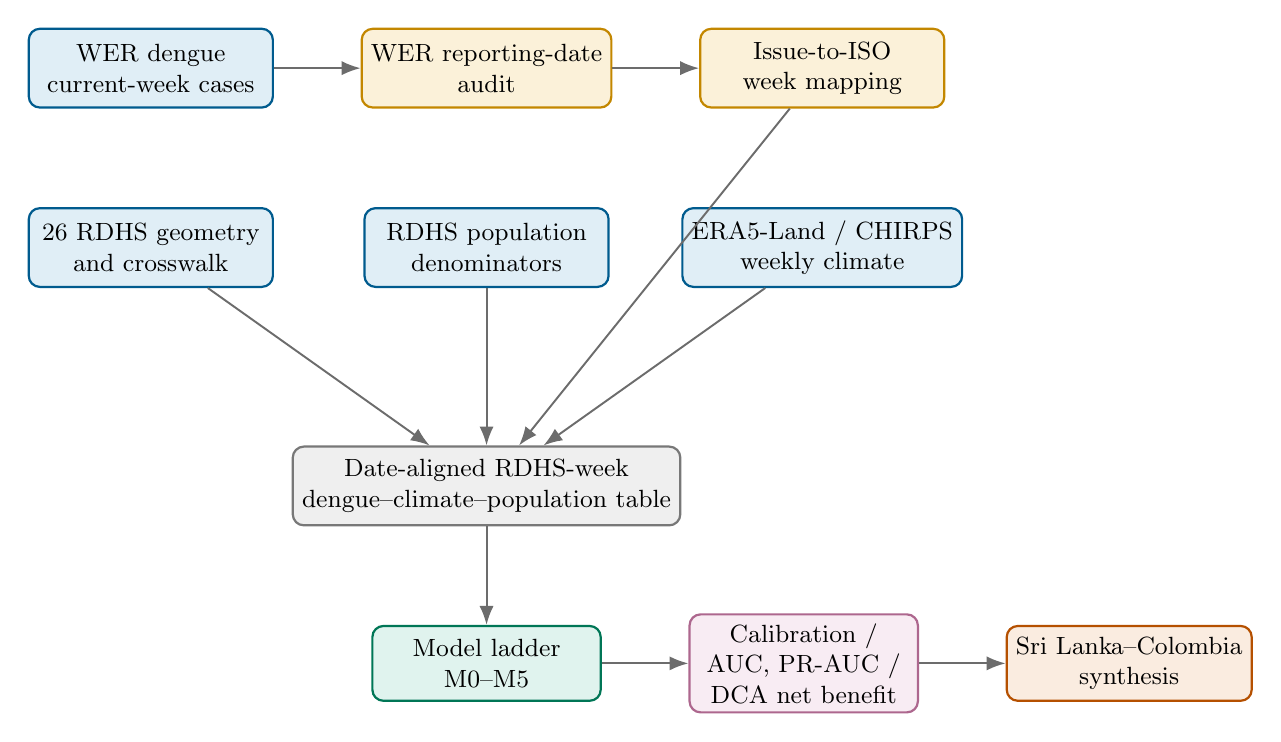
\begin{tikzpicture}[
    node distance=1.25cm and 1.1cm,
    every node/.style={font=\small},
    src/.style   ={rectangle, rounded corners, draw=okBlue!80!black, fill=okBlue!12, line width=0.8pt, align=center, minimum width=3.1cm, minimum height=1.0cm},
    pre/.style   ={rectangle, rounded corners, draw=okOrange!85!black, fill=okOrange!15, line width=0.8pt, align=center, minimum width=3.1cm, minimum height=1.0cm},
    integ/.style ={rectangle, rounded corners, draw=okGray, fill=okGray!12, line width=0.8pt, align=center, minimum width=4.6cm, minimum height=1.0cm},
    mod/.style   ={rectangle, rounded corners, draw=okGreen!75!black, fill=okGreen!12, line width=0.8pt, align=center, minimum width=2.9cm, minimum height=0.95cm},
    evaln/.style ={rectangle, rounded corners, draw=okPurple!85!black, fill=okPurple!14, line width=0.8pt, align=center, minimum width=2.9cm, minimum height=0.95cm},
    outnode/.style={rectangle, rounded corners, draw=okVermillion!85!black, fill=okVermillion!12, line width=0.8pt, align=center, minimum width=2.9cm, minimum height=0.95cm},
    arrow/.style ={-{Latex[length=2.4mm]}, line width=0.7pt, draw=okGray!90!black}
]
\node[src] (wer) {WER dengue\\current-week cases};
\node[pre, right=of wer] (date) {WER reporting-date\\audit};
\node[pre, right=of date] (iso) {Issue-to-ISO\\week mapping};
\node[src, below=of iso] (climate) {ERA5-Land / CHIRPS\\weekly climate};
\node[src, below=of date] (pop) {RDHS population\\denominators};
\node[src, below=of wer] (geom) {26 RDHS geometry\\and crosswalk};
\node[integ, below=2.0cm of pop] (linked) {Date-aligned RDHS-week\\dengue--climate--population table};
\node[mod, below=of linked] (models) {Model ladder\\M0--M5};
\node[evaln, right=of models] (eval) {Calibration /\\AUC, PR-AUC /\\DCA net benefit};
\node[outnode, right=of eval] (synth) {Sri Lanka--Colombia\\synthesis};
\draw[arrow] (wer) -- (date);
\draw[arrow] (date) -- (iso);
\draw[arrow] (iso) -- (linked);
\draw[arrow] (climate) -- (linked);
\draw[arrow] (pop) -- (linked);
\draw[arrow] (geom) -- (linked);
\draw[arrow] (linked) -- (models);
\draw[arrow] (models) -- (eval);
\draw[arrow] (eval) -- (synth);
\end{tikzpicture}
\caption{Study pipeline and WER-to-ISO week alignment. Reporting dates were used to map WER issues to ISO epidemiological weeks before joining dengue, climate, population, and spatial data.}
\label{fig:pipeline}
\end{figure}

\subsection{Sri Lanka primary comparison}
Among the initial M0--M3 benchmark comparison, in the held-out 2023--2025 test period the recent-case surveillance model M1 had the highest discrimination, lowest Brier score, and highest net benefit at $p^*=0.30$ (Table~\ref{tab:slprimary}). The climate-only and structured-climate models showed predictive signal but did not exceed M1. At $p^*=0.30$, M1 net benefit was 0.137, versus 0.069 (M2) and 0.078 (M3); alert-all was lower than M1 and alert-none was zero. Decision value was threshold-dependent (Table~\ref{tab:slthresh}, Fig~\ref{fig:sldca}): at low thresholds alert-all was competitive, as expected when the threshold lies well below test prevalence, while across the mid-to-high range M1 was consistently highest among M0--M3.

\begin{table}[htbp]
\centering
\caption{Initial Sri Lanka M0--M3 benchmark comparison ($h=4$, RDHS 75th-percentile alert label, 2023--2025 test period). Hybrid models M4--M5 are reported separately.}
\label{tab:slprimary}
\begin{threeparttable}\footnotesize
\setlength{\tabcolsep}{3.6pt}
\begin{tabular}{llrrrrrrrr}
\toprule
Model & Description & AUC & PR-AUC & Brier & CITL & Slope & Mean pred. & Obs. & NB$_{0.30}$ \\
\midrule
M0 & Seasonal climatology & 0.629 & 0.459 & 0.222 & +0.530 & 0.664 & 0.238 & 0.336 & 0.084 \\
M1 & Recent-case surveillance & 0.752 & 0.652 & 0.191 & +0.513 & 1.246 & 0.246 & 0.336 & 0.137 \\
M2 & Climate-only & 0.643 & 0.460 & 0.220 & +0.479 & 1.027 & 0.243 & 0.336 & 0.069 \\
M3 & Climate + season + RDHS FE & 0.652 & 0.476 & 0.220 & +0.596 & 0.738 & 0.229 & 0.336 & 0.078 \\
\bottomrule
\end{tabular}
\begin{tablenotes}\footnotesize
\item AUC, area under the receiver-operating characteristic curve; PR-AUC, area under the precision--recall curve; Brier, Brier score; CITL, calibration-in-the-large; Slope, calibration slope; Mean pred., mean predicted probability; Obs., observed prevalence; NB$_{0.30}$, net benefit at the primary reference threshold $p^*=0.30$; FE, fixed effects.
\end{tablenotes}
\end{threeparttable}
\end{table}

\begin{table}[htbp]
\centering
\caption{Sri Lanka net benefit at representative decision thresholds.}
\label{tab:slthresh}
\small
\begin{tabular}{rrrrrrr}
\toprule
Threshold $p^*$ & Alert-all & Alert-none & M0 & M1 & M2 & M3 \\
\midrule
0.20 & 0.171 & 0.000 & 0.161 & 0.185 & 0.164 & 0.147 \\
0.30 & 0.052 & 0.000 & 0.084 & 0.137 & 0.069 & 0.078 \\
0.34 & $-0.005$ & 0.000 & 0.059 & 0.111 & 0.032 & 0.060 \\
0.40 & $-0.106$ & 0.000 & 0.025 & 0.083 & 0.012 & 0.039 \\
\bottomrule
\end{tabular}
\end{table}

\begin{figure}[htbp]
\centering
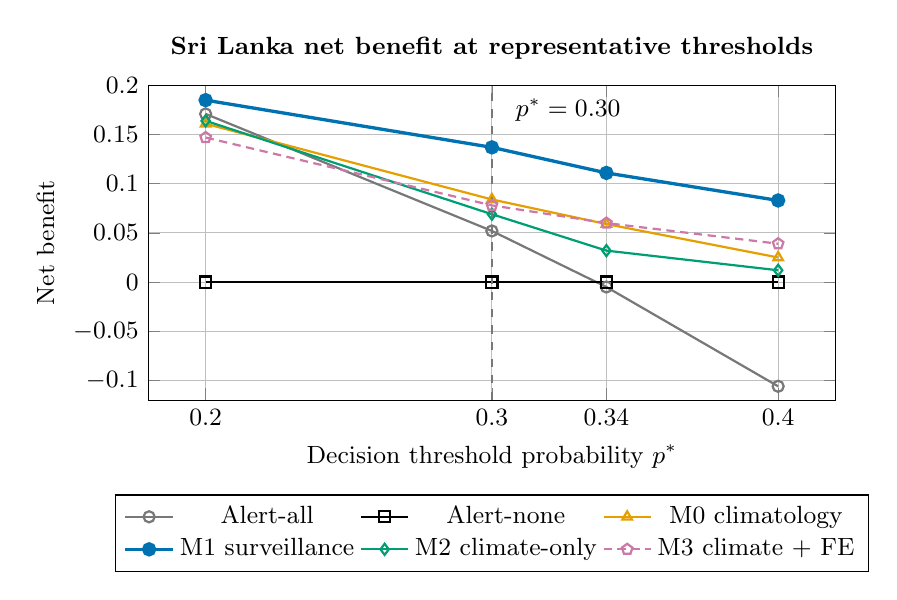
\begin{tikzpicture}
\begin{axis}[
    width=0.85\textwidth, height=0.46\textwidth,
    xlabel={Decision threshold probability $p^*$}, ylabel={Net benefit},
    xmin=0.18, xmax=0.42, ymin=-0.12, ymax=0.20,
    xtick={0.20,0.30,0.34,0.40}, ytick={-0.10,-0.05,0,0.05,0.10,0.15,0.20},
    grid=both, tick label style={font=\small}, label style={font=\small},
    legend style={at={(0.5,-0.30)}, anchor=north, legend columns=3, font=\small},
    title={Sri Lanka net benefit at representative thresholds}, title style={font=\small\bfseries}]
\addplot+[mark=o, thick, color=okGray] coordinates {(0.20,0.171)(0.30,0.052)(0.34,-0.005)(0.40,-0.106)}; \addlegendentry{Alert-all}
\addplot+[mark=square, thick, color=black] coordinates {(0.20,0)(0.30,0)(0.34,0)(0.40,0)}; \addlegendentry{Alert-none}
\addplot+[mark=triangle, thick, color=okOrange] coordinates {(0.20,0.161)(0.30,0.084)(0.34,0.059)(0.40,0.025)}; \addlegendentry{M0 climatology}
\addplot+[mark=*, very thick, color=okBlue] coordinates {(0.20,0.185)(0.30,0.137)(0.34,0.111)(0.40,0.083)}; \addlegendentry{M1 surveillance}
\addplot+[mark=diamond, thick, color=okGreen] coordinates {(0.20,0.164)(0.30,0.069)(0.34,0.032)(0.40,0.012)}; \addlegendentry{M2 climate-only}
\addplot+[mark=pentagon, thick, color=okPurple] coordinates {(0.20,0.147)(0.30,0.078)(0.34,0.060)(0.40,0.039)}; \addlegendentry{M3 climate + FE}
\addplot[dashed, thick, color=okGray] coordinates {(0.30,-0.12)(0.30,0.20)};
\node[anchor=west, font=\small] at (axis cs:0.305,0.175) {$p^*=0.30$};
\end{axis}
\end{tikzpicture}
\caption{Sri Lanka net benefit at representative decision thresholds ($h=4$, 75th-percentile label). Points are net benefit at four representative thresholds (Table~\ref{tab:slthresh}); line segments connect them and do not represent a recomputed continuous grid. The 0.34 threshold brackets the alert-all zero-crossing (alert-all net benefit $-0.005$ there, near the test prevalence of 0.336) and is included as a representative diagnostic threshold, not a selected operating point. The recent-case surveillance model (M1) had the highest net benefit at $p^*=0.30$ and across the evaluated mid-to-high threshold range. Colorblind-safe (Okabe--Ito) palette.}
\label{fig:sldca}
\end{figure}

\subsection{Calibration and recalibration}
All M0--M3 models in the initial comparison under-predicted in the test period (CITL $+0.530$ M0, $+0.513$ M1, $+0.479$ M2, $+0.596$ M3; mean predicted $\approx$0.23--0.25 against observed prevalence 0.336), consistent with the 24.2\%$\rightarrow$33.6\% training-to-test prevalence shift. The hybrid models M4 and M5 also under-predicted in the test period (CITL $+0.449$ and $+0.440$, calibration slopes 1.225 and 1.077), so the under-prediction was not confined to the initial benchmark ladder. Rolling 52-week intercept-only recalibration substantially reduced calibration-in-the-large error for all models, leaving residual CITL of $+0.029$ (M0), $+0.020$ (M1), $+0.046$ (M2), and $+0.087$ (M3) (Table~\ref{tab:recal}), and outperformed expanding-window recalibration, which under-corrected. Intercept-only recalibration addresses average under- or over-prediction but does not by itself correct calibration slope or nonlinear miscalibration, so it does not imply perfect calibration; for example, M3's residual CITL was $+0.087$. No recalibration fallbacks occurred. Recalibration did not change the model ranking: across the evaluated recalibration methods M1 net benefit at $p^*=0.30$ ranged 0.124--0.142 while the maximum recalibrated climate-only (M2/M3) net benefit was approximately 0.085, so reducing calibration error did not make climate-only models exceed surveillance.

\begin{table}[htbp]
\centering
\caption{Calibration-in-the-large before and after time-updated recalibration.}
\label{tab:recal}
\small
\begin{tabular}{lrrrr}
\toprule
Model & Raw CITL & Rolling-52 & Rolling-104 & Expanding \\
\midrule
M0 & +0.530 & +0.029 & +0.137 & +0.338 \\
M1 & +0.513 & +0.020 & +0.111 & +0.325 \\
M2 & +0.479 & +0.046 & +0.155 & +0.314 \\
M3 & +0.596 & +0.087 & +0.204 & +0.394 \\
\bottomrule
\end{tabular}
\end{table}

\subsection{Sri Lanka structured-climate and hybrid results}
The Python DLNM-style and canonical R \texttt{dlnm} climate specifications produced nearly identical performance: the Python DLNM-style minus canonical R-DLNM differences in AUC and in net benefit at $p^*=0.30$ were near zero. Both climate specifications remained below the recent-surveillance benchmark M1. For the canonical R DLNM minus M1, the canonical R-DLNM estimates were lower than M1 by 0.038 in AUC (95\% CI $-0.066$ to $-0.008$) and by 0.025 in net benefit at $p^*=0.30$ (95\% CI $-0.041$ to $-0.006$) (M1 net benefit 0.137 versus 0.112 for the canonical R DLNM) (Table~\ref{tab:dlnmhybrid}). For the initially planned Sri Lanka hybrid, the M4$-$M1 net-benefit estimate at $p^*=0.30$ was $-0.008$ (95\% CI $-0.028$ to $+0.013$) and $\Delta$AUC(M4$-$M1) was $+0.013$ (95\% CI $-0.020$ to $+0.046$). The expanded hybrid M5 (adding seasonal harmonics and geographic fixed effects to M4) reached AUC 0.772, PR-AUC 0.667, Brier 0.180 (CITL $+0.440$, calibration slope 1.077; M4 CITL $+0.449$, slope 1.225), and net benefit 0.145 at $p^*=0.30$ (M1: 0.752, 0.652, 0.191, 0.137); the M5$-$M1 net-benefit estimate at $p^*=0.30$ was $+0.0081$ (95\% CI $-0.0012$ to $+0.0181$), a small positive point estimate with substantial uncertainty (Table~\ref{tab:dlnmhybrid}; see the cross-setting summary).

\begin{table}[htbp]
\centering
\caption{Sri Lanka climate-only, distributed-lag, and hybrid model comparison (test period, $h=4$, 75th-percentile label). Net benefit is shown at representative thresholds. M4 is the initially planned hybrid; M5 is the expanded hybrid (adding seasonal harmonics and geographic fixed effects to M4).}
\label{tab:dlnmhybrid}
\small
\begin{tabular}{lrrrr}
\toprule
Model & AUC & NB$_{0.20}$ & NB$_{0.30}$ & NB$_{0.40}$ \\
\midrule
M1 recent-case surveillance & 0.752 & 0.185 & 0.137 & 0.083 \\
M2 climate-only & 0.643 & 0.164 & 0.069 & 0.012 \\
M3 climate + season/RDHS & 0.652 & 0.147 & 0.078 & 0.039 \\
Python DLNM-style climate & 0.714 & 0.179 & 0.111 & 0.057 \\
Canonical R DLNM climate & 0.714 & 0.181 & 0.112 & 0.053 \\
M4 initially planned hybrid & 0.764 & 0.193 & 0.128 & 0.087 \\
M5 expanded hybrid & 0.772 & 0.194 & 0.145 & 0.107 \\
\bottomrule
\end{tabular}
\end{table}

\subsection{Colombia external framework replication}
The Colombia primary $h=4$ analysis used a common-complete test set (n${}=13{,}361$; test prevalence 0.375) on which models M0--M5 were all evaluated, with the complete-case intersection defined by the M1--M5 predictors; the split was training 2006--2017, validation 2018--2019, and test 2020--2022. As in Sri Lanka, climate-only models were weak (M2 AUC 0.556, M3 0.564) relative to M1 (AUC 0.685). The hybrid had a higher net-benefit point estimate than M1: M5 AUC 0.726 and net benefit 0.136 at $p^*=0.30$ versus M1 0.685 and 0.117, with municipality-cluster bootstrap $\Delta$AUC $+0.040$ (95\% CI $+0.024$ to $+0.058$) and $\Delta$NB at $p^*=0.30$ $+0.0188$ (95\% CI $+0.0117$ to $+0.0260$) (Table~\ref{tab:colombia}, Fig~\ref{fig:colombia}). At $p^*=0.30$, the $\Delta$NB of $+0.0188$ corresponds to approximately 1.9 additional net true-positive equivalents per 100 municipality-weeks (approximate interval 1.2 to 2.6 per 100). Equivalently---rather than additionally---holding true-positive detections fixed, it corresponds to approximately 4.4 fewer false-alert equivalents per 100 municipality-weeks (approximate interval 2.7 to 6.1 per 100). Both intervals are monotone rescalings of the same pointwise, multiplicity-unadjusted $\Delta$NB confidence interval and inherit its caveats. These are alternative decision-analytic representations of the same net-benefit difference, not observed numbers of outbreaks detected, alerts prevented, cases prevented, or lives saved. The Colombia test period (2020--2022) includes the COVID-19-era years 2020--2021. Platt recalibration was fit on the validation period, and the calibration metrics reported here are after that recalibration. All models nonetheless over-predicted in the test period: calibration-in-the-large remained negative for every model (M0 $-0.50$, M1 $-0.46$, M2 $-0.50$, M3 $-0.54$, M4 $-0.45$, M5 $-0.50$), with Brier scores 0.213--0.250, consistent with the temporal prevalence shift not being fully removed by validation-fit recalibration. Colombia calibration slopes ranged from 0.85 to 3.43 across the model ladder; the extremes were the climatology baseline M0 (slope 3.43) and the climate-only baseline M2 (slope 0.85), whereas the models carrying the net-benefit comparison---M1, M4, and M5---had slopes near 1 (1.09, 1.05, and 1.16). M0, M2 and M3 had net benefit approximately equal to the alert-all strategy and below M1, M4 and M5. Although M1 and M5 were evaluated on the same test observations and under the same validation-fit recalibration framework, both retained test-period calibration error. Their net-benefit contrast should therefore be interpreted together with the reported calibration-in-the-large, calibration-slope and Brier-score results. Observed prevalence was 0.375 for the common-complete test set, which was shared by all models; per-model mean predicted probability was not retained in the committed reproducibility record. The within-test M5-versus-M1 contrast is reported with this calibration limitation.

\begin{table}[htbp]
\centering
\caption{Colombia $h=4$ primary common-complete test performance (external framework replication). Net benefit at $p^*=0.30$; alert-all reference $\approx$0.107, alert-none $0$. Test prevalence was 0.375 for the common-complete set shared by M0--M5. Per-model mean predicted probabilities were not retained in the committed reproducibility record. Calibration-in-the-large, calibration slope, and Brier-score results are summarized in the text and Supporting Information.}
\label{tab:colombia}
\small
\begin{tabular}{llrr}
\toprule
Model & Description & AUC & NB$_{0.30}$ \\
\midrule
M0 & Seasonal climatology & 0.513 & 0.108 \\
M1 & Recent-case surveillance & 0.685 & 0.117 \\
M2 & Climate-only & 0.556 & 0.108 \\
M3 & Climate + seasonality + department fixed effects & 0.564 & 0.108 \\
M4 & Recent cases + linear climate lags (no seasonality or fixed effects) & 0.699 & 0.129 \\
M5 & Hybrid climate + surveillance & 0.726 & 0.136 \\
\midrule
\multicolumn{2}{l}{Alert-all reference} & --- & $\approx$0.107 \\
\bottomrule
\end{tabular}
\end{table}

\noindent In the primary common-complete analysis, M2 and M3 had net benefit close to alert-all ($\approx$0.107) and below M1. In a separate, larger climate-only row set their net benefit was approximately 0.001 (AUC $\approx$0.532 and 0.546), indicating that climate-only weakness was not an artifact of the common-complete subset. Because the analyses used different denominators, they are reported separately.

\begin{figure}[htbp]
\centering
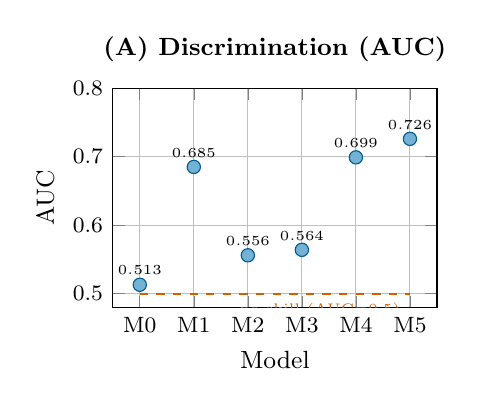
\begin{tikzpicture}
\begin{axis}[
    width=0.47\textwidth, height=0.36\textwidth,
    symbolic x coords={M0,M1,M2,M3,M4,M5}, xtick=data, ymin=0.48, ymax=0.80, ytick={0.5,0.6,0.7,0.8},
    ylabel={AUC}, xlabel={Model}, grid=both,
    tick label style={font=\footnotesize}, label style={font=\small},
    title={(A) Discrimination (AUC)}, title style={font=\small\bfseries},
    nodes near coords, every node near coord/.append style={font=\tiny, anchor=south},
    nodes near coords style={/pgf/number format/.cd, fixed, precision=3}]
\draw[dashed, thick, draw=okVermillion] ({axis cs:M0,0.5}) -- ({axis cs:M5,0.5});
\node[anchor=north east, font=\tiny, text=okVermillion] at (axis cs:M5,0.5) {no-skill (AUC$=$0.5)};
\addplot[only marks, mark=*, mark size=2.4pt, draw=okBlue!80!black, fill=okBlue!55] coordinates {(M0,0.513)(M1,0.685)(M2,0.556)(M3,0.564)(M4,0.699)(M5,0.726)};
\end{axis}
\end{tikzpicture}\hfill
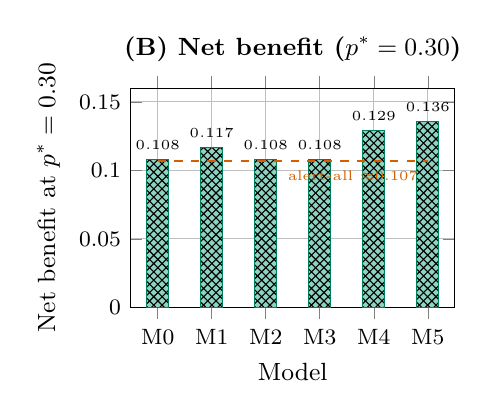
\begin{tikzpicture}
\begin{axis}[
    width=0.47\textwidth, height=0.36\textwidth, ybar, bar width=8pt,
    symbolic x coords={M0,M1,M2,M3,M4,M5}, xtick=data, ymin=0, ymax=0.16, ytick={0,0.05,0.10,0.15},
    ylabel={Net benefit at $p^*=0.30$}, xlabel={Model}, grid=both,
    tick label style={font=\footnotesize}, label style={font=\small},
    title={(B) Net benefit ($p^*=0.30$)}, title style={font=\small\bfseries},
    nodes near coords, every node near coord/.append style={font=\tiny},
    nodes near coords style={/pgf/number format/.cd, fixed, precision=3}]
\addplot[fill=okGreen!45, draw=okGreen!80!black, postaction={pattern=crosshatch}] coordinates {(M0,0.108)(M1,0.117)(M2,0.108)(M3,0.108)(M4,0.129)(M5,0.136)};
\draw[dashed, thick, draw=okVermillion] ({axis cs:M0,0.107}) -- ({axis cs:M5,0.107});
\node[anchor=north east, font=\tiny, text=okVermillion] at (axis cs:M5,0.107) {alert-all $\approx$0.107};
\end{axis}
\end{tikzpicture}
\caption{Colombia model-ladder discrimination and net benefit ($h=4$, common-complete test set, $n=13{,}361$). (A) AUC and (B) net benefit at $p^*=0.30$ for models M0--M5. Panel~A is a dot plot with a dashed reference line at the no-skill value (AUC${}=0.5$), the meaningful baseline for discrimination, with exact three-decimal AUC values labeled above each point (no truncated bars). Panel B uses a zero-based axis so that the alert-none reference (net benefit $=0$) is the baseline and the alert-all reference ($\approx$0.107, dashed line) and the small between-model differences are shown in true proportion; exact three-decimal values are labeled above each bar. Climate-only models (M2, M3) had net benefit close to alert-all and below M1; M5 had the highest AUC and net benefit. Values are transcribed from Table~\ref{tab:colombia}; Panel~B bars use a redundant hatch pattern and Panel~A uses filled circular markers for grayscale legibility.}
\label{fig:colombia}
\end{figure}

\subsection{Horizon result}
Across the tested Colombia horizons, the M5$-$M1 net-benefit increment was approximately flat rather than increasing with lead time: $\Delta$NB(M5$-$M1) was approximately $+0.015$ to $+0.019$ across $h=1$--8 and approximately $+0.014$ at $h=12$, while $\Delta$AUC fell from approximately $+0.040$ ($h\le4$) to approximately $+0.024$ ($h=12$). In Sri Lanka, the recent-surveillance baseline (M1) retained the highest net benefit at $p^*=0.30$ across the evaluated label--horizon cells; M1 discrimination declined with horizon (AUC 0.843, 0.810, 0.752, 0.679, 0.646 at $h=1,2,4,8,12$ for the 75th-percentile label), with climate models narrowing the discrimination gap at long horizons as M1's own discrimination decayed, without overturning the net-benefit result. The Sri Lanka and Colombia horizon analyses estimate related but not identical quantities. Together, these findings provided no evidence that climate delivered increasing decision value over the tested 1--12-week range.

\subsection{Threshold and stricter-outcome robustness}
In Sri Lanka, a secondary targeted-value analysis across train-defined regimes found the all-test $\Delta$NB(M5$-$M1) at $p^*=0.30$ was $+0.0081$ (95\% CI $-0.0012$ to $+0.0181$); the regime estimates were small with wide, pointwise, multiplicity-unadjusted intervals, and the largest regime estimate (high-incidence $\times$ strong-autocorrelation, $+0.0202$, 95\% CI $+0.0038$ to $+0.0370$) was interpreted as exploratory and imprecise because it was based on only eight clusters. At $p^*=0.40$, the all-test $\Delta$NB(M5$-$M1) estimate was $+0.0241$ (95\% CI $+0.0090$ to $+0.0399$), compared with $+0.0081$ at the primary reference threshold of $p^*=0.30$ and $+0.0096$ (95\% CI $-0.0005$ to $+0.0187$) at $p^*=0.20$. This was a secondary threshold-specific analysis; the evaluated-grid estimates were pointwise and unadjusted for multiplicity. Incremental net benefit was larger at the higher evaluated threshold ($p^*=0.40$) than at $p^*=0.30$ or $p^*=0.20$, although these secondary estimates are interpreted descriptively rather than as separate hypothesis tests; the complete evaluated grid is transcribed in the threshold-grid traceability record. In Colombia, the secondary stricter exceedance-threshold sensitivity (training-referenced 75th/80th/90th-percentile labels) gave $\Delta$NB(M5$-$M1) at $p^*=0.30$ of $+0.0188$ (95\% CI $+0.0117$ to $+0.0260$), $+0.0157$ (95\% CI $+0.0082$ to $+0.0236$), and $+0.0092$ (95\% CI $+0.0003$ to $+0.0183$); the estimates attenuated from $+0.0188$ at the 75th-percentile definition to $+0.0092$ at the 90th-percentile definition, and all intervals are pointwise and unadjusted for multiplicity. Even at the 90th-percentile definition the test-period prevalence of elevated-activity weeks remained approximately 23.5\%, so these are not evidence for rare-epidemic prediction. The 75th-percentile $h=4$ contrast remains the primary analysis; its operational translation is reported in the primary Colombia Results above.

\subsection{Cross-setting synthesis}
The Sri Lanka and Colombia hybrid estimates are shown side by side in Table~\ref{tab:crosssetting}. In Sri Lanka, the M5$-$M1 net-benefit estimate was $+0.0081$, with a 95\% CI from $-0.0012$ to $+0.0181$. In Colombia, the corresponding estimate was $+0.0188$, with a 95\% CI from $+0.0117$ to $+0.0260$. No cross-country interaction or heterogeneity test was designed or performed; therefore, the study does not establish that the setting-specific estimates differ. Recent surveillance was a strong benchmark in both settings; climate-only models added limited decision value in both; and the hybrid increment was modest and varied in magnitude and precision across the evaluated settings.

\begin{table}[htbp]
\centering
\caption{Cross-setting hybrid increment, $\Delta$NB(M5$-$M1) at $p^*=0.30$ (primary $h=4$, 75th-percentile label). 95\% CIs are percentile bootstrap and pointwise. No cross-country interaction or heterogeneity test was performed. The estimates therefore should not be interpreted as establishing a between-setting difference. The settings differ in period, spatial units, sample size, and climate-feature implementation.}
\label{tab:crosssetting}
\small
\begin{tabular}{lrr}
\toprule
Setting & $\Delta$NB(M5$-$M1) & 95\% CI \\
\midrule
Sri Lanka (RDHS-cluster bootstrap, all-test) & +0.0081 & $-0.0012$ to $+0.0181$ \\
Colombia (municipality-cluster bootstrap) & +0.0188 & $+0.0117$ to $+0.0260$ \\
\bottomrule
\end{tabular}
\end{table}

% =====================================================================
% DISCUSSION
% =====================================================================
\section{Discussion}

The principal evaluation lesson is that climate-informed dengue early-warning models should be evaluated against recent surveillance and judged using calibration and decision-curve net benefit, not discrimination alone. Under that standard, recent surveillance was a strong benchmark in both settings. Climate-only models added limited decision value, while hybrid models showed a modest incremental signal whose magnitude and precision varied across the evaluated settings. In Colombia, the M5$-$M1 net-benefit increment remained approximately flat across the evaluated horizons; in Sri Lanka, M1 retained the highest net benefit across the evaluated label--horizon cells. These analyses addressed related but not identical quantities. The flat Colombia increment runs counter to the common expectation that climate information becomes more valuable at longer lead times as the recent-case signal decays; here it did not grow with horizon, which is itself informative for prioritizing surveillance inputs in short-to-medium-term alerting. Formal between-country heterogeneity was not tested. Throughout, the recent-case benchmark M1 is a locally refit statistical model, not the deployed early-warning and response system we cite as motivation~\cite{EWARScsd}; ``hard to beat'' refers to this statistical baseline. The alert target is an elevated-activity flag (roughly a third of weeks), not a rare-outbreak declaration, so the evaluation concerns elevated-activity alerting rather than rare-epidemic early warning.

The limited decision value of the climate-only models should not be read as climate being irrelevant to transmission. Recent case counts already summarize upstream processes, including climate effects, so over short-to-medium horizons a recent-case baseline is a demanding but appropriate comparator, and even a canonical distributed-lag nonlinear climate model did not exceed it at the primary threshold. The hybrid results are the key nuance: the M5$-$M1 estimate was $+0.0081$ (95\% CI $-0.0012$ to $+0.0181$) in Sri Lanka and $+0.0188$ (95\% CI $+0.0117$ to $+0.0260$) in Colombia. No between-country heterogeneity test was performed, so the two settings are best read as complementary rather than contradictory and do not establish a difference: climate value may be conditional on setting, surveillance dynamics, and outcome and threshold definitions, and is most defensible as an incremental signal within a hybrid system that requires local evaluation. The magnitude of the Colombia increment was modest: at $p^*=0.30$ it corresponds to approximately 1.9 net true-positive equivalents (approximate interval 1.2 to 2.6) per 100 municipality-weeks, or, at a fixed number of true-positive detections, approximately 4.4 fewer false-alert equivalents (approximate interval 2.7 to 6.1) per 100 --- decision-analytic representations of the same net-benefit difference, not observed public-health outcomes.

Two practical evaluation lessons deserve emphasis. First, the date-aligned WER-to-ISO linkage mattered: a naive week-number join would have misaligned climate exposure and dengue outcomes by one to two weeks, which could bias conclusions about lagged climate associations. Second, decision-curve net benefit and calibration revealed patterns that discrimination alone would obscure. Calibration drift was substantial in the test period. Rolling 52-week intercept-only recalibration reduced, but did not eliminate, average miscalibration (for example, M3 residual calibration-in-the-large was $+0.087$). It did not correct calibration slope or nonlinear miscalibration and did not change the model ranking. These patterns argue for ongoing calibration monitoring in any operational use rather than a one-time check.

Several limitations bound these conclusions. The study was retrospective, used finalized rather than real-time surveillance counts, and did not simulate reporting delay. Because both recent-case predictors and the eventual alert outcome are derived from surveillance counts, reporting delays and later revisions could affect predictor availability, outcome ascertainment, and the estimated M5$-$M1 contrast. The direction and magnitude of this effect cannot be determined from finalized retrospective data. Climate-product availability and latency were not evaluated in this study. The Colombia test period was 2020--2022 and therefore includes the COVID-19-era years 2020--2021; finalized (rather than real-time) reporting and pandemic-era disruption may affect absolute calibration and comparative performance, and a pandemic-period exclusion analysis was not performed in the current study, so its effect on the M5$-$M1 contrast cannot be inferred. We do not treat the current estimate as a lower bound. Alert labels were percentile (exceedance) thresholds rather than official outbreak declarations, the primary Sri Lanka design used a single temporal holdout rather than a rolling-origin and spatial-block design, climate exposures were aggregated to administrative units (raising change-of-support and modifiable-areal-unit concerns), and the settings differed in surveillance periods, spatial units, sample sizes, climate-feature implementation, and validation design, which limits direct cross-setting comparison. Colombia is external framework replication, not external model validation, so the findings do not establish that coefficients or thresholds transport to other settings, and we make no claim of deployment readiness, transportability, causal climate effects, cost-effectiveness, rare-epidemic prediction, or universal hybrid benefit. Future work should evaluate the framework prospectively under real-time reporting and connect decision thresholds to explicit costs and losses. Mechanistically motivated climate--transmission modeling would require additional serotype, immunity, entomological, mobility, intervention, and reporting-process data and is reserved for separate work.

In summary, recent dengue surveillance is a strong operational benchmark, climate-only models add limited standalone decision value, and climate may add a modest increment within hybrid systems whose magnitude and precision varied across the evaluated settings. Operational evaluations should report calibration and decision-curve net benefit against recent-surveillance baselines before claims of climate-informed value are made.

% =====================================================================
% DECLARATIONS (placeholders; mirror the standalone draft files)
% =====================================================================
\section*{Declarations}
\textbf{Ethics.} The study used aggregate, publicly accessible surveillance data. A formal institutional determination is pending author/institutional confirmation.\\
\textbf{Data and code availability.} Public source datasets (OpenDengue, CHIRPS, ERA5-Land, WorldPop, WER) are cited. Repository and archival details (repository URL, persistent identifier, license) are pending author confirmation.\\
\textbf{Funding.} Pending author confirmation.\\
\textbf{Competing interests.} Pending author confirmation.\\
\textbf{Author contributions.} Pending author confirmation.\\
\textbf{Acknowledgments.} Pending author confirmation.\\
\textbf{Use of AI assistance.} During preparation of this study, the authors used Anthropic Claude through the Claude Code interface under author supervision to assist with drafting and reviewing analysis code, executing prespecified computational workflows, organizing and checking outputs against frozen analysis reports, auditing references, preparing documentation, and editing manuscript language and structure. The authors determined the study questions and analysis decisions, reviewed the code and outputs, independently checked the reported results and citations, and take full responsibility for the accuracy and integrity of the work. The AI system was not listed as an author and did not independently make final scientific or publication decisions.

% =====================================================================
% REFERENCES (Vancouver numbered)
% =====================================================================
% Vancouver-style references, numbered by order of appearance (NLM journal
% abbreviations; first six authors then et al. for >6). Authored inline as a
% thebibliography (no Vancouver .bst is installed) and generated from
% references_v7.bib; renders without BibTeX.
\begingroup
\setstretch{1.0}
\begin{thebibliography}{99}
\setlength{\itemsep}{2pt}

\bibitem{Mordecai2017} Mordecai EA, Cohen JM, Evans MV, Gudapati P, Johnson LR, Lippi CA, et al. Detecting the impact of temperature on transmission of Zika, dengue, and chikungunya using mechanistic models. PLoS Negl Trop Dis. 2017;11(4):e0005568. doi:\,10.1371/journal.pntd.0005568.

\bibitem{Huber2018} Huber JH, Childs ML, Caldwell JM, Mordecai EA. Seasonal temperature variation influences climate suitability for dengue, chikungunya, and Zika transmission. PLoS Negl Trop Dis. 2018;12(5):e0006451. doi:\,10.1371/journal.pntd.0006451.

\bibitem{Johansson2019} Johansson MA, Apfeldorf KM, Dobson S, Devita J, Buczak AL, Baugher B, et al. An open challenge to advance probabilistic forecasting for dengue epidemics. Proc Natl Acad Sci U S A. 2019;116(48):24268--24274. doi:\,10.1073/pnas.1909865116.

\bibitem{Baharom2022} Baharom M, Ahmad N, Hod R, Abdul Manaf MR. Dengue early warning system as outbreak prediction tool: a systematic review. Risk Manag Healthc Policy. 2022;15:871--886. doi:\,10.2147/RMHP.S361106.

\bibitem{HussainAlkhateeb2021} Hussain-Alkhateeb L, Rivera Ramirez T, Kroeger A, Gozzer E, Runge-Ranzinger S. Early warning systems (EWSs) for chikungunya, dengue, malaria, yellow fever, and Zika outbreaks: what is the evidence? A scoping review. PLoS Negl Trop Dis. 2021;15(9):e0009686. doi:\,10.1371/journal.pntd.0009686.

\bibitem{Lowe2021} Lowe R, Lee SA, O'Reilly KM, Brady OJ, Bastos L, Carrasco-Escobar G, et al. Combined effects of hydrometeorological hazards and urbanisation on dengue risk in Brazil: a spatiotemporal modelling study. Lancet Planet Health. 2021;5(4):e209--e219. doi:\,10.1016/S2542-5196(20)30292-8.

\bibitem{VanCalster2019} Van Calster B, McLernon DJ, van Smeden M, Wynants L, Steyerberg EW. Calibration: the Achilles heel of predictive analytics. BMC Med. 2019;17:230. doi:\,10.1186/s12916-019-1466-7.

\bibitem{VanCalster2023} Van Calster B, Steyerberg EW, Wynants L, van Smeden M. There is no such thing as a validated prediction model. BMC Med. 2023;21:70. doi:\,10.1186/s12916-023-02779-w.

\bibitem{SteyerbergVergouwe2014} Steyerberg EW, Vergouwe Y. Towards better clinical prediction models: seven steps for development and an ABCD for validation. Eur Heart J. 2014;35(29):1925--1931. doi:\,10.1093/eurheartj/ehu207.

\bibitem{Vickers2006} Vickers AJ, Elkin EB. Decision curve analysis: a novel method for evaluating prediction models. Med Decis Making. 2006;26(6):565--574. doi:\,10.1177/0272989X06295361.

\bibitem{Vickers2016} Vickers AJ, Van Calster B, Steyerberg EW. Net benefit approaches to the evaluation of prediction models, molecular markers, and diagnostic tests. BMJ. 2016;352:i6. doi:\,10.1136/bmj.i6.

\bibitem{Vickers2019} Vickers AJ, van Calster B, Steyerberg EW. A simple, step-by-step guide to interpreting decision curve analysis. Diagn Progn Res. 2019;3:18. doi:\,10.1186/s41512-019-0064-7.

\bibitem{Murphy1985} Murphy AH. Decision making and the value of forecasts in a generalized model of the cost-loss ratio situation. Mon Weather Rev. 1985;113(3):362--369. doi:\,10.1175/1520-0493(1985)113\textless0362:DMATVO\textgreater2.0.CO;2.

\bibitem{Tozan2023} Tozan Y, Sewe MO, Kim S, Rockl\"ov J. A methodological framework for economic evaluation of operational response to vector-borne diseases based on early warning systems. Am J Trop Med Hyg. 2023;108(3):627--633. doi:\,10.4269/ajtmh.22-0471.

\bibitem{EWARScsd} Schlesinger M, Prieto Alvarado FE, Borb\'on Ramos ME, Sewe MO, Merle CS, Kroeger A, et al. Enabling countries to manage outbreaks: statistical, operational, and contextual analysis of the early warning and response system (EWARS-csd) for dengue outbreaks. Front Public Health. 2024;12:1323618. doi:\,10.3389/fpubh.2024.1323618.

\bibitem{vonElm2007} von Elm E, Altman DG, Egger M, Pocock SJ, G\o tzsche PC, Vandenbroucke JP. The Strengthening the Reporting of Observational Studies in Epidemiology (STROBE) statement: guidelines for reporting observational studies. Lancet. 2007;370(9596):1453--1457. doi:\,10.1016/S0140-6736(07)61602-X.

\bibitem{Collins2024TRIPODAI} Collins GS, Dhiman P, Navarro CL, Ma J, Hooft L, Reitsma JB, et al. TRIPOD+AI statement: updated guidance for reporting clinical prediction models that use regression or machine learning methods. BMJ. 2024;385:e078378. doi:\,10.1136/bmj-2023-078378.

\bibitem{Wolff2019} Wolff RF, Moons KGM, Riley RD, Whiting PF, Westwood M, Collins GS, et al. PROBAST: a tool to assess the risk of bias and applicability of prediction model studies. Ann Intern Med. 2019;170(1):51--58. doi:\,10.7326/M18-1376.

\bibitem{Moons2019} Moons KGM, Wolff RF, Riley RD, Whiting PF, Westwood M, Collins GS, et al. PROBAST: a tool to assess risk of bias and applicability of prediction model studies: explanation and elaboration. Ann Intern Med. 2019;170(1):W1--W33. doi:\,10.7326/M18-1377.

\bibitem{HDXCODABSriLanka} Humanitarian Data Exchange, OCHA, Survey Department of Sri Lanka. Sri Lanka administrative boundaries (COD-AB) [dataset]. Humanitarian Data Exchange; 2022.

\bibitem{SriLankaWER} Epidemiology Unit, Ministry of Health, Sri Lanka. Weekly Epidemiological Report: dengue current-week case tables [Internet]. Colombo: Ministry of Health; 2018--2025.

\bibitem{Clarke2024OpenDengue} Clarke J, Lim A, Gupte P, Pigott DM, van Panhuis WG, Brady OJ. A global dataset of publicly available dengue case count data. Sci Data. 2024;11:296. doi:\,10.1038/s41597-024-03120-7.

\bibitem{OpenDengue2024} OpenDengue. Global dengue data, Temporal extract [dataset]. figshare; 2025. doi:\,10.6084/m9.figshare.24259573.

\bibitem{Tatem2017} Tatem AJ. WorldPop, open data for spatial demography. Sci Data. 2017;4:170004. doi:\,10.1038/sdata.2017.4.

\bibitem{WorldPop2025} WorldPop. Global 2015--2030 population data, R2025A, 100\,m [dataset]. Southampton: University of Southampton; 2025.

\bibitem{SriLankaCensus2025} Department of Census and Statistics, Sri Lanka. Census of Population and Housing 2024: basic population information by districts and DS divisions. Battaramulla: Department of Census and Statistics; 2025.

\bibitem{MunozSabater2021} Mu\~noz-Sabater J, Dutra E, Agust\'i-Panareda A, Albergel C, Arduini G, Balsamo G, et al. ERA5-Land: a state-of-the-art global reanalysis dataset for land applications. Earth Syst Sci Data. 2021;13:4349--4383. doi:\,10.5194/essd-13-4349-2021.

\bibitem{ERA5LandCDS} Copernicus Climate Change Service. ERA5-Land hourly data from 1950 to present [dataset]. Copernicus Climate Data Store; 2019. doi:\,10.24381/cds.e2161bac.

\bibitem{Funk2015} Funk C, Peterson P, Landsfeld M, Pedreros D, Verdin J, Shukla S, et al. The climate hazards infrared precipitation with stations---a new environmental record for monitoring extremes. Sci Data. 2015;2:150066. doi:\,10.1038/sdata.2015.66.

\bibitem{CHIRPS} Climate Hazards Center, University of California Santa Barbara. CHIRPS: Climate Hazards Group InfraRed Precipitation with Station data [dataset]. Santa Barbara: University of California; 2015.

\bibitem{Gasparrini2010} Gasparrini A, Armstrong B, Kenward MG. Distributed lag non-linear models. Stat Med. 2010;29(21):2224--2234. doi:\,10.1002/sim.3940.

\bibitem{Gasparrini2011} Gasparrini A. Distributed lag linear and non-linear models in R: the package dlnm. J Stat Softw. 2011;43(8):1--20. doi:\,10.18637/jss.v043.i08.

\bibitem{RCoreTeam2026} R Core Team. R: a language and environment for statistical computing. Version 4.6.0. Vienna: R Foundation for Statistical Computing; 2026.

\bibitem{SaitoRehmsmeier2015} Saito T, Rehmsmeier M. The precision-recall plot is more informative than the ROC plot when evaluating binary classifiers on imbalanced datasets. PLoS One. 2015;10(3):e0118432. doi:\,10.1371/journal.pone.0118432.

\bibitem{CameronGelbachMiller2008} Cameron AC, Gelbach JB, Miller DL. Bootstrap-based improvements for inference with clustered errors. Rev Econ Stat. 2008;90(3):414--427. doi:\,10.1162/rest.90.3.414.

\end{thebibliography}
\endgroup

% =====================================================================
% SUPPORTING INFORMATION CAPTIONS (after References, standard order)
% =====================================================================
\clearpage
\section*{Supporting information}
\begingroup\setstretch{1.0}
\noindent All items below exist as standalone files transcribed from frozen committed reports (no recomputation). Checklists S1--S3 and the inventory S10 remain drafts pending author finalization; S4--S9 are complete and awaiting author approval. No item is submission-final until the declarations and checklists are completed (see the Supporting-Information status record and \texttt{submission\_blockers\_v7.md}).\\[0.4em]
\noindent\textbf{S1 Checklist.} STROBE checklist for observational studies (draft).\\
\textbf{S2 Checklist.} TRIPOD+AI reporting checklist; records that flexible graphical calibration curves were not generated (draft internal aid).\\
\textbf{S3 Table.} PROBAST risk-of-bias domain assessment (draft internal aid).\\
\textbf{S4 Text.} Analysis-plan and addendum chronology, including the M4 (initially planned) / M5 (expanded) hybrid designation.\\
\textbf{S5 Table.} Per-country M0--M5 model specification, events-per-variable, and software versions (R~4.6.0, \texttt{dlnm}~2.4.10, \texttt{mgcv}~1.9.4, \texttt{tsModel}~0.6-2 verified; Python modeling-stack versions not preserved).\\
\textbf{S6 Table.} Per-analysis bootstrap protocol (resampling unit, $B$, interval method, degenerate-resample handling, failure count; seeds where retained).\\
\textbf{S7 Table.} Sri Lanka linkage, climate-lag, and late-2021 anomaly sensitivity grid.\\
\textbf{S8 Table.} Sri Lanka targeted-value regime analysis.\\
\textbf{S9 Table.} Colombia exceedance-threshold (75th/80th/90th) and horizon sensitivity.\\
\textbf{S10 Text.} Reproducibility-artifact inventory and checksums (partial; author to finalize).
\endgroup

\end{document}
